\newpage
\partie{3}
\section{Sportifs Qui Ont Un Age Entre 20 Et 30}

\vspace{0.25cm}
\textbf{\underline{Code}}
\lstinputlisting{Parties/Partie3/q12.sql}


\vspace{0.25cm}
\textbf{\underline{Output}}

\vspace{0.25cm}
\begin{center}
    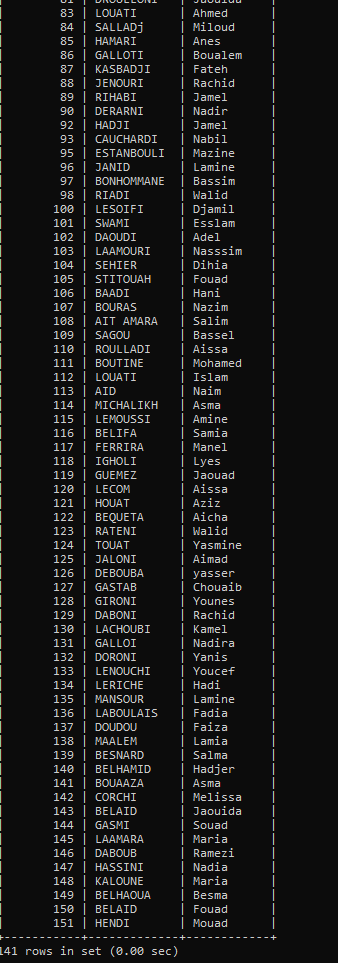
\includegraphics[height=0.6\textheight]{Parties/Partie3/sportifs.PNG}
\end{center}

\newpage

\section{Les Conseillers}
\vspace{0.25cm}
\textbf{\underline{Code}}
\lstinputlisting{Parties/Partie3/q13.sql}


\vspace{0.25cm}
\textbf{\underline{Output}}

\vspace{0.25cm}
\begin{center}
    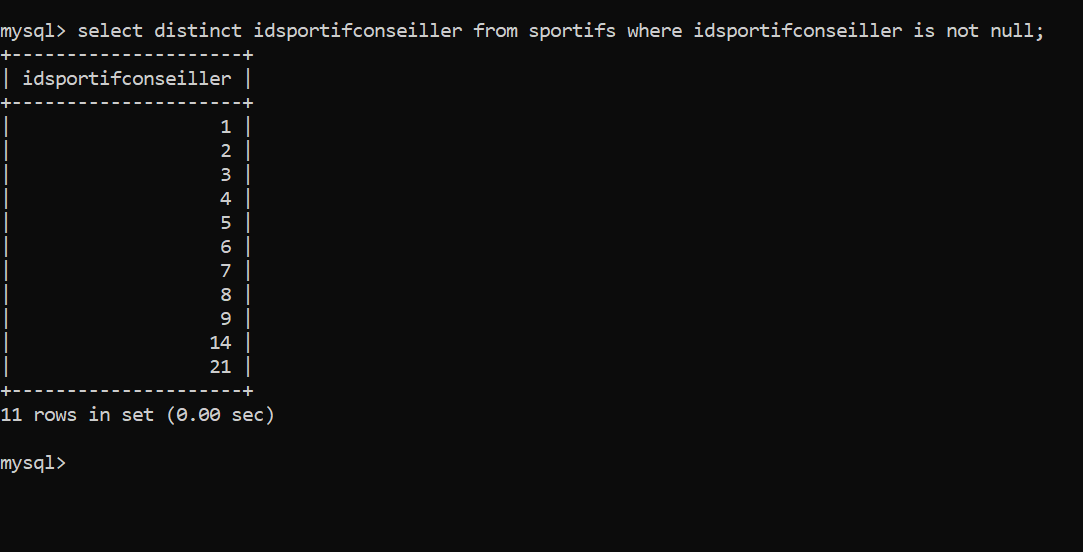
\includegraphics[width=0.8\textwidth]{Parties/Partie3/conseiller.PNG}
\end{center}

\vspace{0.25cm}
\begin{prettyBox}{Remarque}{red}
On a utilise \textcolor{blue}{DISTINCT} parceque l'attribut \texttt{IdSportifConseiller} est une
cle strangere donc elle peut etre repete sure plusieur lignes , et on a verifie si l'id ete \textcolor{blue}{NULL} ,
pour filtrer les valeur \textcolor{blue}{NULL} (sportifs sans conseiller)
\end{prettyBox}

\newpage
\section{Entraineur De Hand-Ball Ou Basket-Ball}

\begin{prettyBox}{Explication}{myblue}
\textbf{\underline{Soit Hand-Ball, Soit Basket-Ball, Ou Les Deux}} \\[0.15cm]
On a un \textcolor{blue}{SELECT} imbriqué où la subquery nous donne les \texttt{IdSportifEntraineur}
qui n'ont pas entraîné au moins une foit 'Hand-Ball' ou 'Basket-Ball',  
en effectuant une jointure entre les tables \texttt{Entrainer} et \texttt{Sports} avec
un \textcolor{blue}{NOT IN} pour récupérer les \texttt{LIBELLE}.  
L'outer query sélectionne les \texttt{IdSportifEntraineur} qui ne font pas partie de cet ensemble,  
ce qui revient à obtenir les entraîneurs qui pratiquent exclusivement le Hand-Ball ,le Basket-Ball, ou les deux.
\vspace{0.25cm}

\textbf{\underline{Soit Hand-Ball, Soit Basket-Ball Uniquement}} \\[0.15cm]
Même logique, sauf que cette fois, on utilise deux requêtes avec \textcolor{blue}{UNION} :  
la première récupère les IDs des entraîneurs qui ne pratiquent aucun sport autre que le Hand-Ball,  
et la seconde ceux qui ne pratiquent aucun sport autre que le Basket-Ball.  
La différence réside dans l'ensemble utilisé dans le \textcolor{blue}{NOT IN}.
\end{prettyBox}
\vspace{0.5cm}
\textbf{\underline{Code}}
\lstinputlisting{Parties/Partie3/q14.sql}

\vspace{0.5cm}
\textbf{\underline{Output}}

\vspace{0.25cm}
\begin{center}
    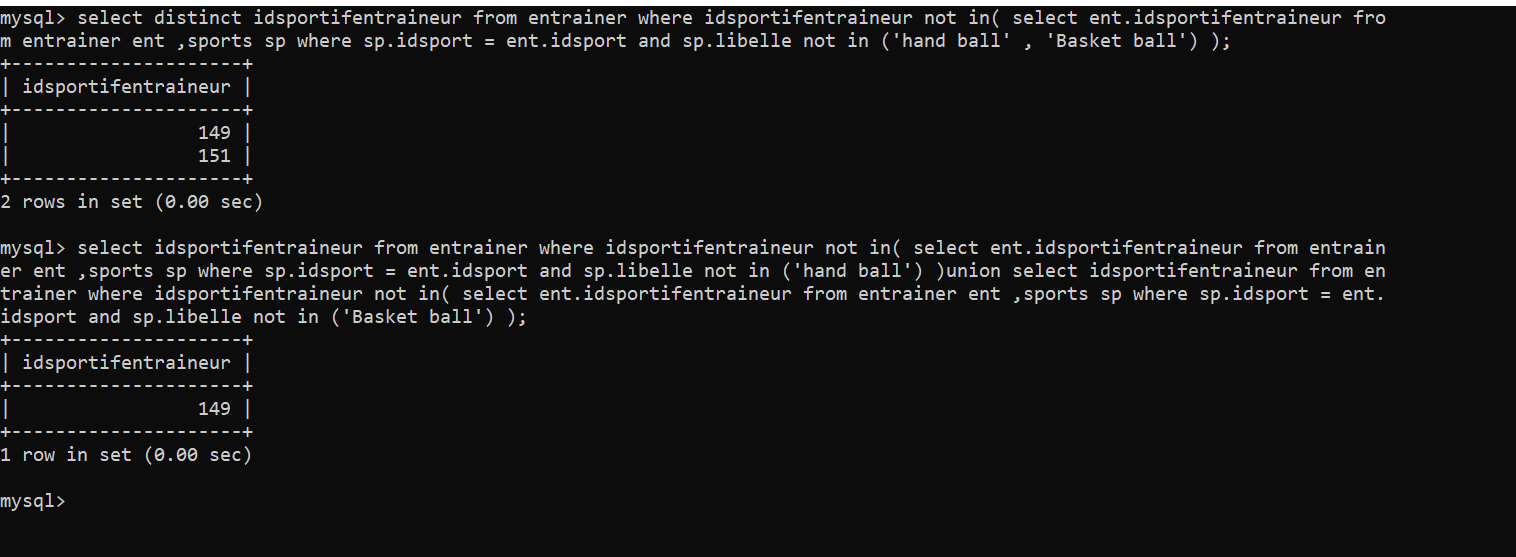
\includegraphics[width=0.8\textwidth]{Parties/Partie3/ent.PNG}
\end{center}

\newpage

\section{Sportifs Les Plus jeunes}

\textbf{\underline{Code}}
\lstinputlisting{Parties/Partie3/q15.sql}

\vspace{0.5cm}
\textbf{\underline{Output}}

\vspace{0.25cm}
\begin{center}
    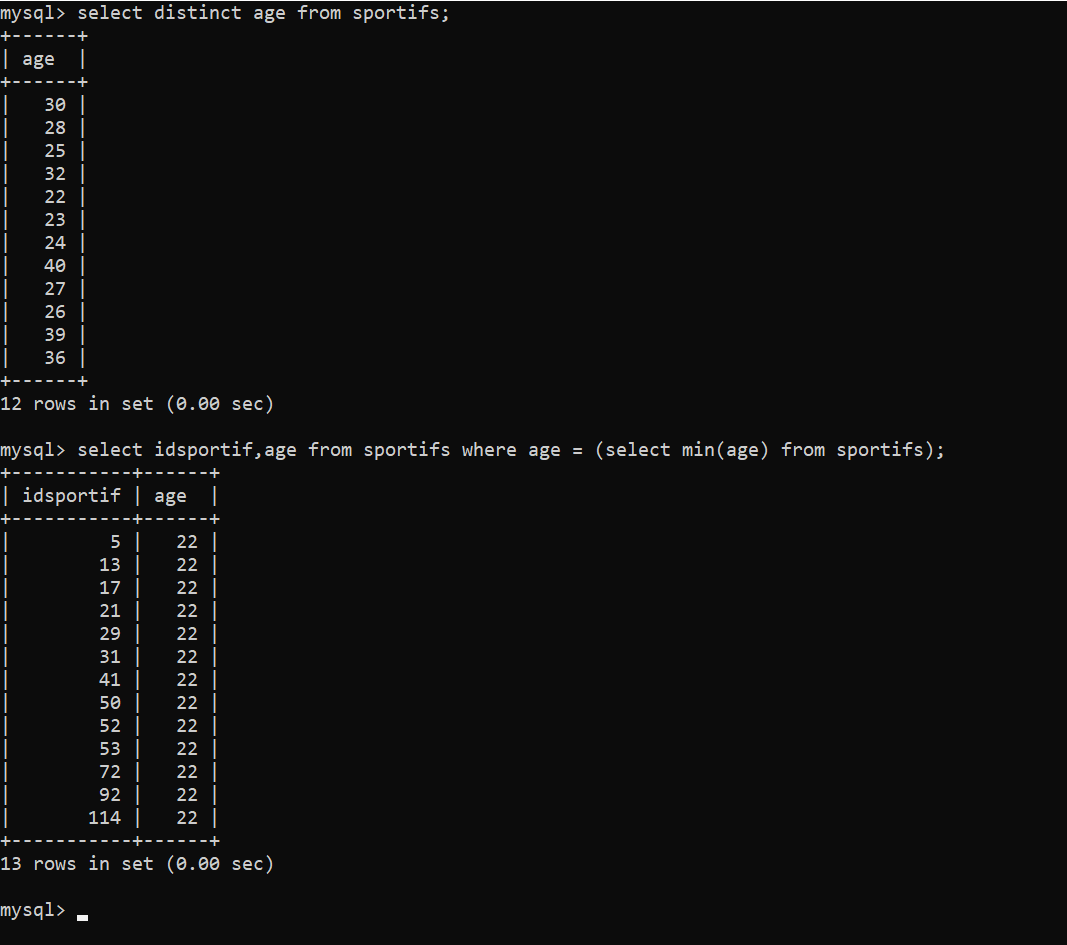
\includegraphics[width=0.8\textwidth]{Parties/Partie3/age.PNG}
\end{center}

\newpage

\section{Superficie Moyennes Des Gymnases Par Ville}

\textbf{\underline{Code}}
\lstinputlisting{Parties/Partie3/q16.sql}

\vspace{0.5cm}
\textbf{\underline{Output}}

\vspace{0.25cm}
\begin{center}
    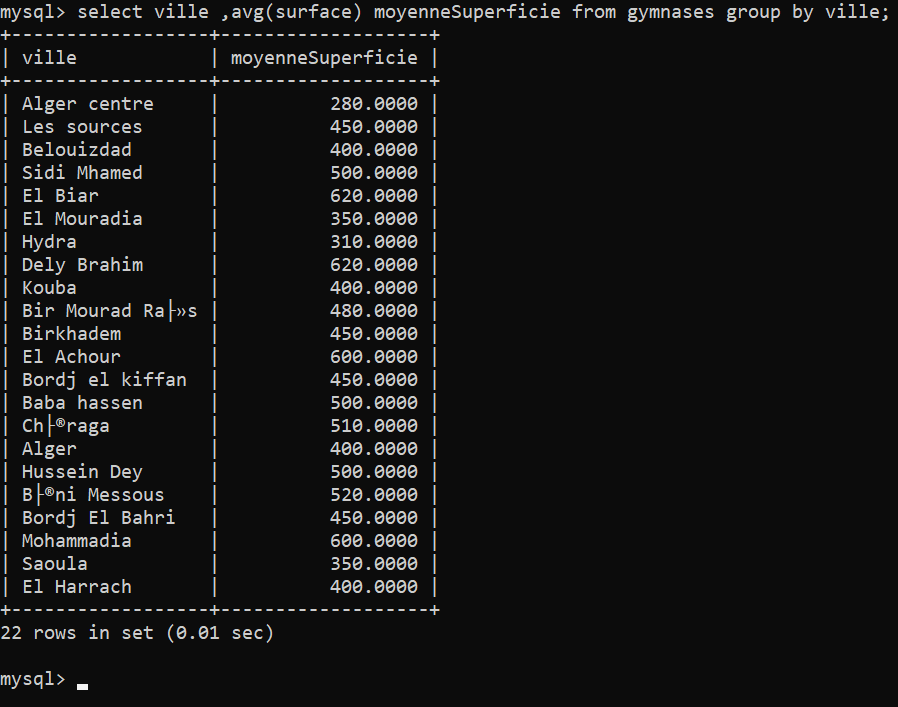
\includegraphics[width=0.8\textwidth]{Parties/Partie3/avg.PNG}
\end{center}

\newpage

\section{Ville Avec Le Plus Grand Nombre De Gymnases}

\textbf{\underline{Code}}
\lstinputlisting{Parties/Partie3/q17.sql}

\vspace{0.5cm}
\textbf{\underline{Output}}

\vspace{0.25cm}
\begin{center}
    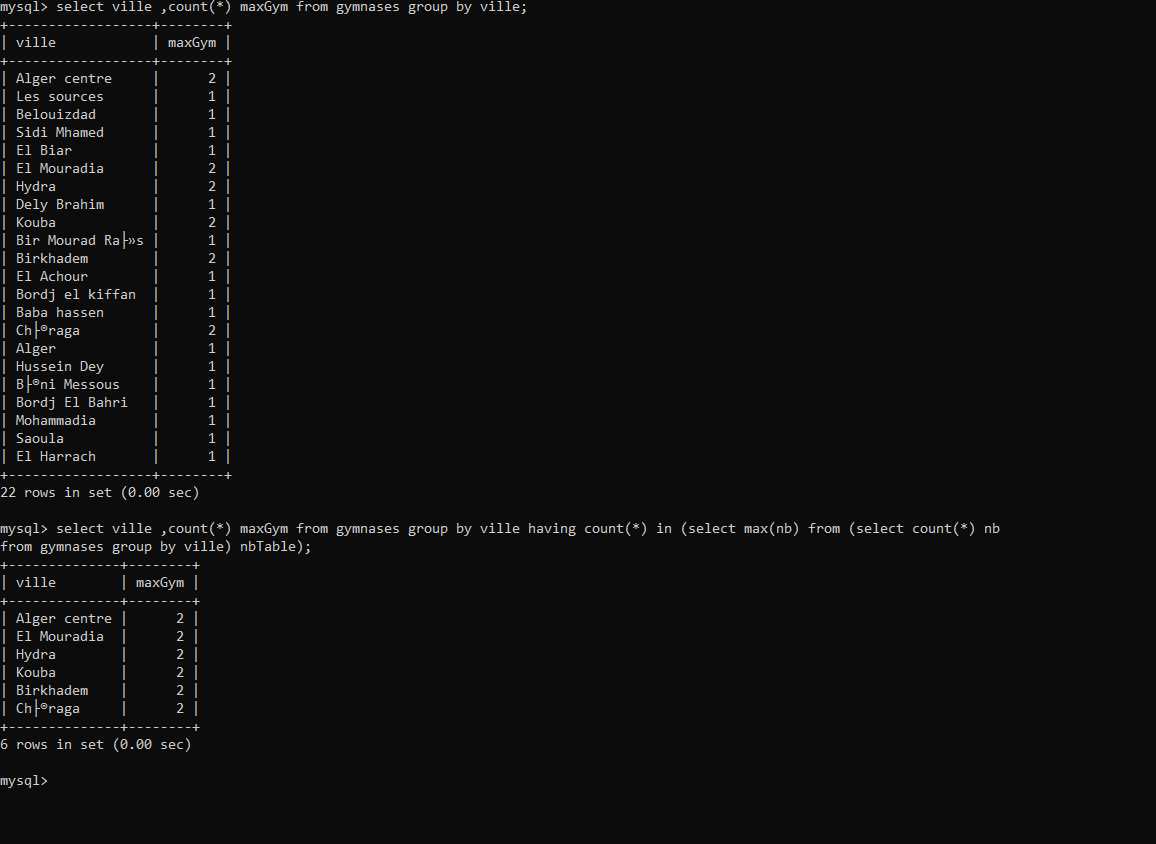
\includegraphics[width=0.8\textwidth]{Parties/Partie3/nbgym.PNG}
\end{center}

\vspace{0.5cm}

\begin{prettyBox}{Note}{red}
On ne peut pas utiliser \textcolor{blue}{COUNT(*)} comme paramètre dans \textcolor{blue}{MAX},  
donc on est obligé d'utiliser une subquery qui génère la table qui contient la colonne des  
nombres de gymnases pour chaque ville.
\end{prettyBox}

